\problemname{Katthalsbandet}
\noindent

\illustration{0.4}{Katthalsbandet.png}{Katten Lulli}

Louise tycker mycket om sin katt Lulli och planterar därför mycket kattmynta.

Nu vill Louise skapa ett fint halsband åt Lulli med $N$ berlocker placerade i en ring.
På varje berlock finns exakt en symbol, antingen \texttt{(} eller \texttt{)}.
Halsbandet har också en bjällra som visar var man börjar läsa.

För att halsbandet ska bli extra fint vill Louise att halsbandet ska vara balanserat.
För att få hjälp anlitar Louise en smyckesmakare som kan bygga om halsbandet. Som betalning använder hon kattmynt.

Smyckesmakaren kan ta bort valfri berlock för en kostnad av $a$ kattmynt per berlock.
Smyckesmakaren kan också vrida halsbandet ett steg, så att den första berlocken i ringen hamnar sist, vilket kostar $b$ kattmynt.
Louise är även nöjd om halsbandet blir helt tomt, men då måste hon betala för att få bort varje berlock.

Louise vill därför göra halsbandet balanserat till så låg kostnad som möjligt.

Ett halsband är balanserat om symbolerna, lästa i ordning från bjällran, bildar en balanserad parentessträng.
En parentessträng är balanserad om:
\begin{itemize}
    \item Den är tom, eller
    \item Den kan skrivas som $AB$, där både $A$ och $B$ är balanserade strängar, eller
    \item Den kan skrivas som $(A)$, där $A$ är en balanserad sträng.
\end{itemize}


\section*{Indata}
Den första raden innehåller tre heltal $N$, $a$ och $b$ ($1 \leq N \leq 5 \cdot 10^5$, $1 \leq a \leq 10^9$, $0 \leq b \leq 10^9$).

Den andra raden innehåller en sträng $s$ av längd $N$.
Varje symbol i $s$ är antingen \texttt{(} eller \texttt{)}.

\section*{Utdata}
Skriv ut ett heltal: den minsta möjliga totalkostnaden för att göra halsbandet balanserat.


\section*{Poängsättning}
Din lösning kommer att testas på en mängd testfallsgrupper.
För att få poäng för en grupp så måste du klara alla testfall i gruppen.

\noindent
\begin{tabular}{| l | l | p{12cm} |}
  \hline
  \textbf{Grupp} & \textbf{Poäng} & \textbf{Gränser} \\ \hline
  $1$    & $5$        & $a = 1, b = 10^9$ \\ \hline
  $2$    & $7$        & $N \le 100$  \\ \hline
  $3$    & $8$        & $N \le 2000$ \\ \hline
  $4$    & $19$       & $b = 0$ \\ \hline
  $5$    & $11$       & $a = 10^9, b = 1$, det finns lika många \texttt{(} som \texttt{)} i indatasträngen. \\ \hline
  $6$    & $14$       & $a = 10^9, b = 1$ \\ \hline
  $7$    & $12$       & Det finns lika många \texttt{(} som \texttt{)} i indatasträngen. \\ \hline
  $8$    & $24$       & Inga ytterligare begränsningar. \\ \hline
\end{tabular}

\section*{Förklaring av exempelfall}
I exempelfall $1$ kan du först vrida halsbandet två steg.
\begin{center}
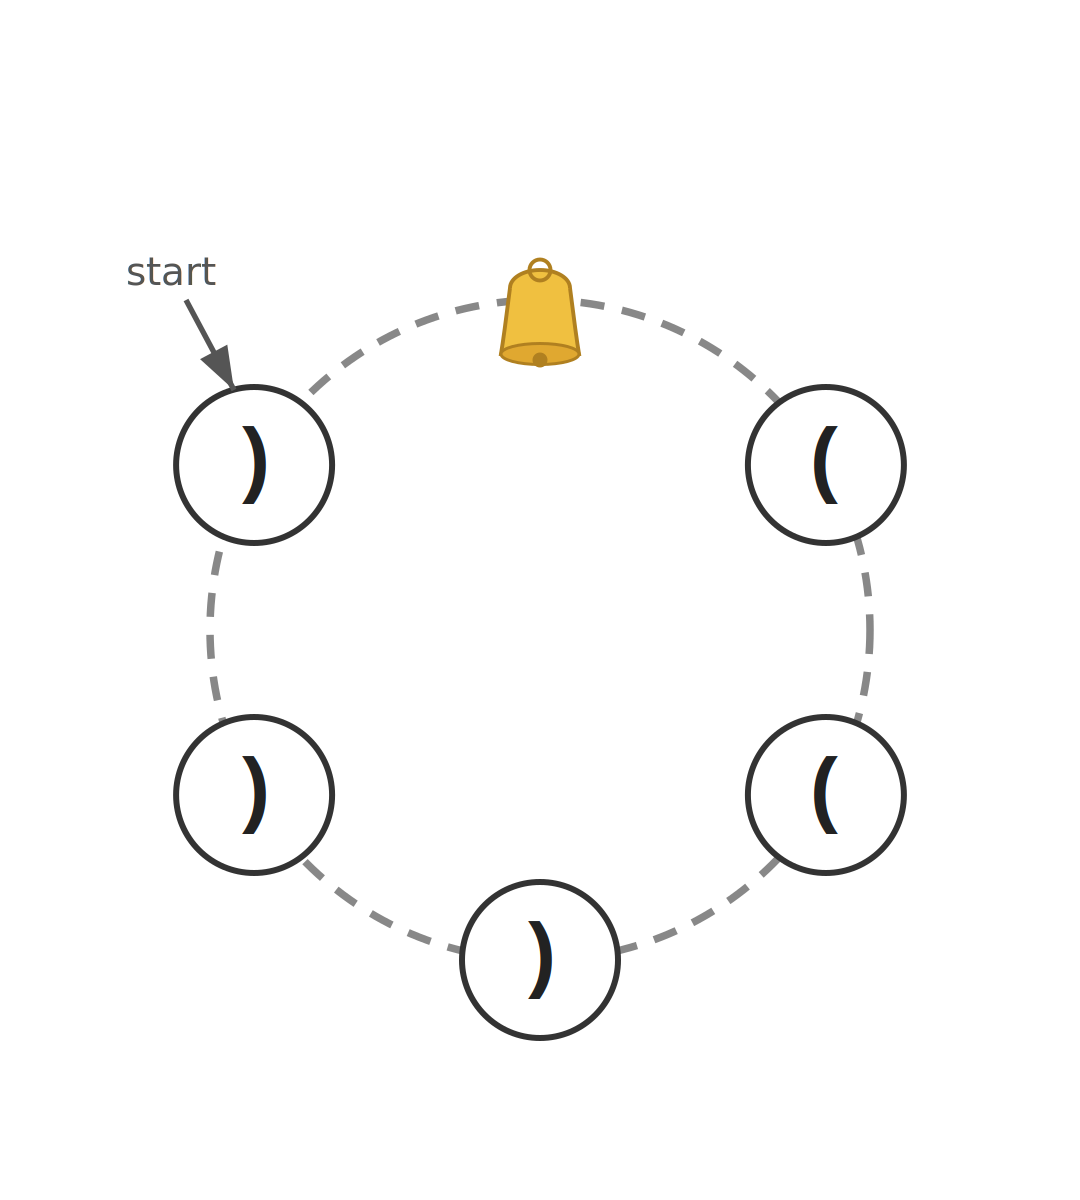
\includegraphics[width=0.5\textwidth]{sample1_1.png}
\end{center}
Då läses halsbandet som \texttt{)(())}.
\begin{center}
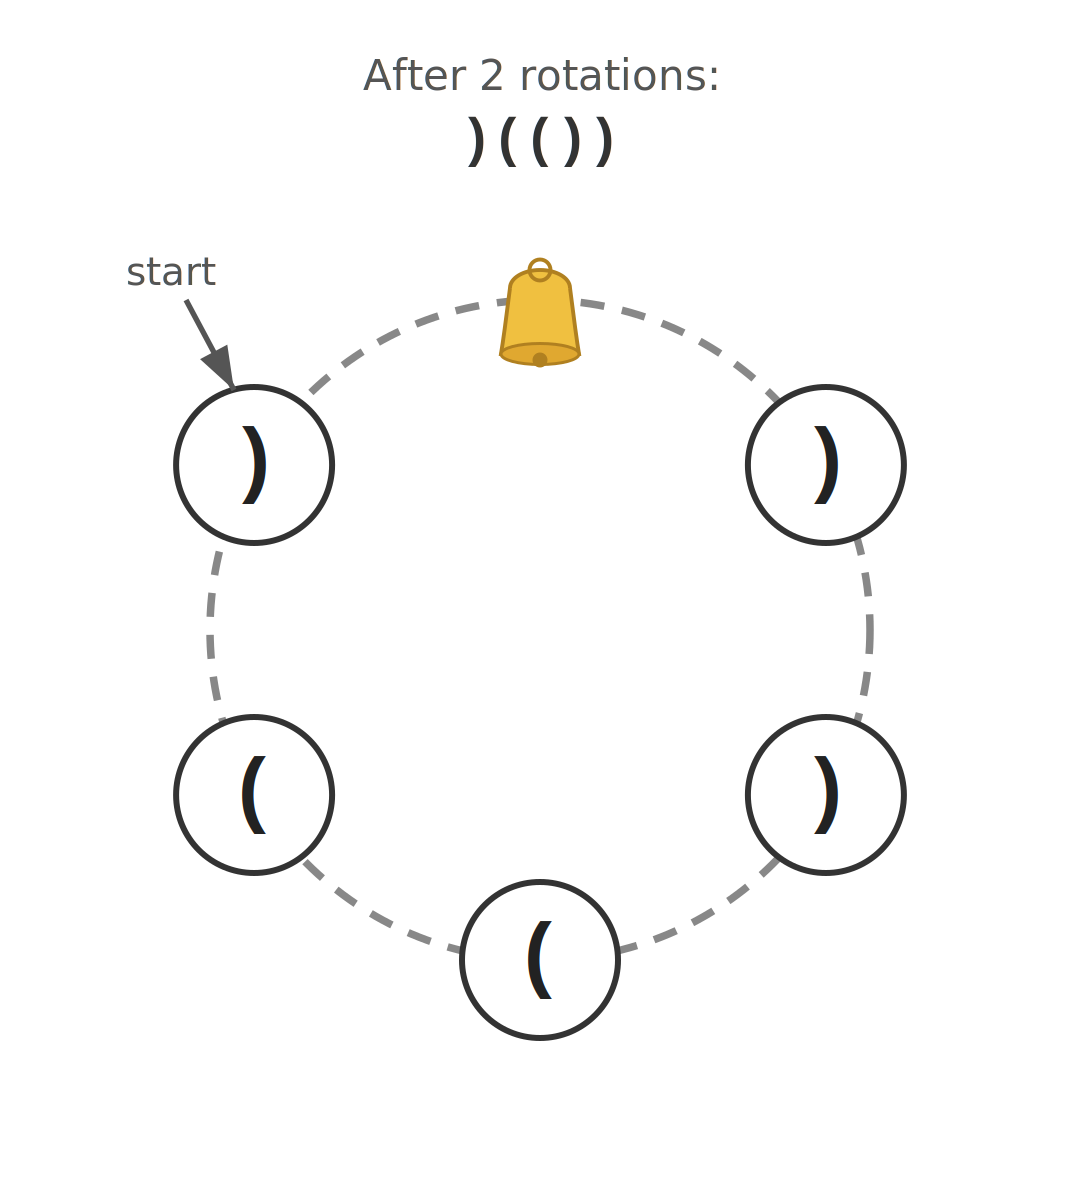
\includegraphics[width=0.5\textwidth]{step1_rotate.png}
\end{center}
Om du sedan tar bort den första berlocken, som är \texttt{)}, läses halsbandet som \texttt{(())}, vilket är balanserat.
\begin{center}
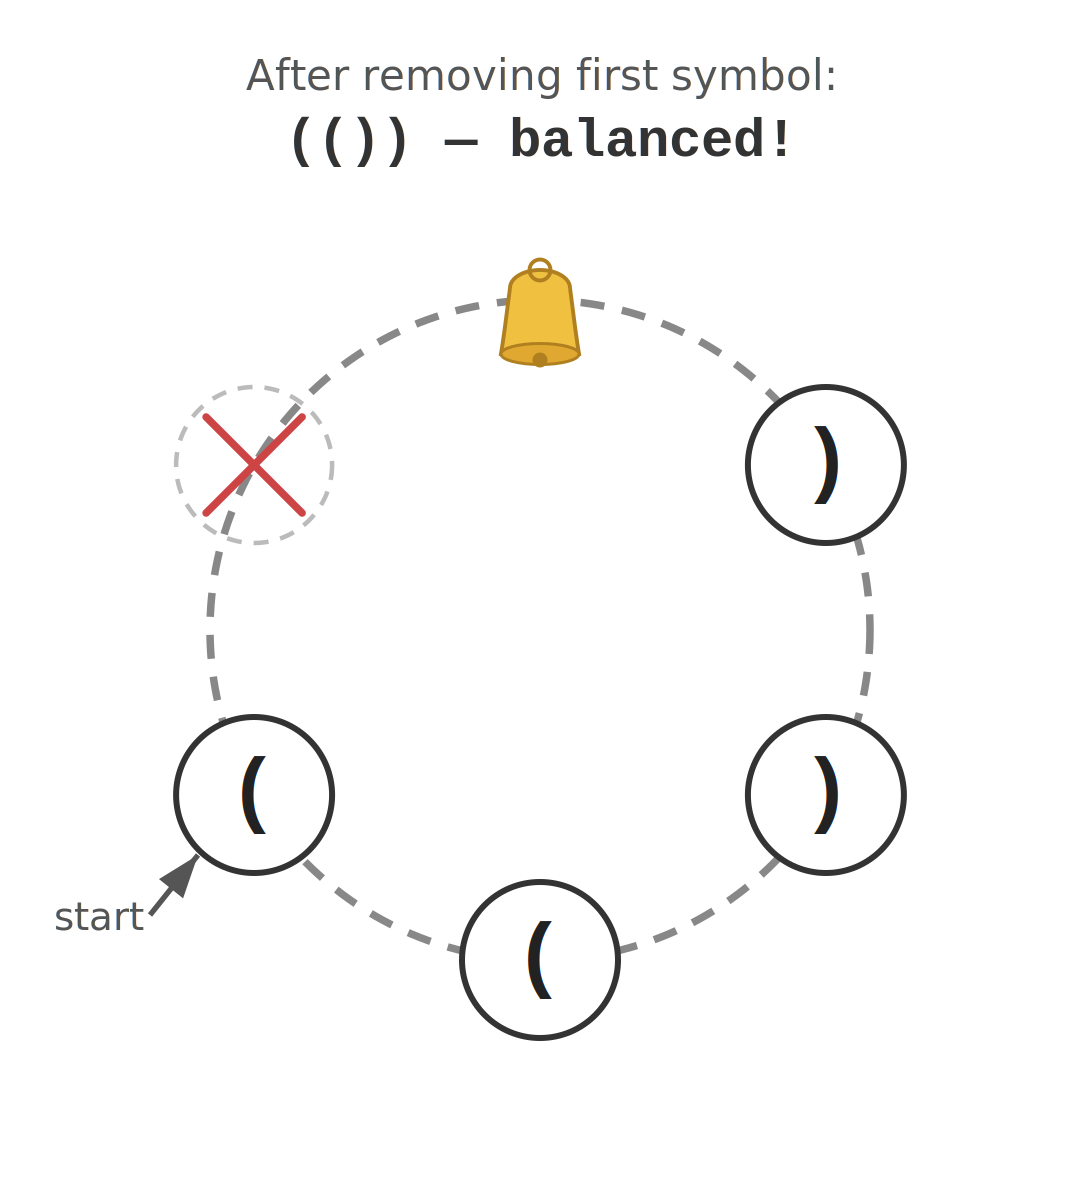
\includegraphics[width=0.5\textwidth]{step2_remove.png}
\end{center}
Den totala kostnaden blir $3 + 3 + 2 = 8$ kattmynt.

I exempelfall $2$ kan du ta bort den andra berlocken, som är \texttt{)}, och därefter den sista berlocken, som är \texttt{(}.
Då läses halsbandet som \texttt{()()()}, vilket är balanserat.
Den totala kostnaden blir $4 + 4 = 8$ kattmynt.

I exempelfall $3$ kan du vrida halsbandet tre steg, så att halsbandet läses som \texttt{()()(())}.
Det är redan balanserat, så den totala kostnaden blir $3 + 3 + 3 = 9$ kattmynt.
